\pagenumbering{roman}
\begin{appendices}
% \addcontentsline{toc}{part}{\appendixname}
% \chapter{Evaluation System Usability Scale}
\chapter{User Evaluation}


\section{Task Sheet}

\subsection*{Task 0 - Joining the Slack workspace}
    
\begin{enumerate}
    \item Use the following link
    to join the Slack workspace if you are not a member yet
    \url{https://join.slack.com/t/mensacommunity/shared_invite/zt-nf09nfmb-EsChPf76BwKsUUlaRJqFqw}
    % \begin{figure}[h]
    %     \centering
    %     
\includegraphics[height=7cm]{../presentation/frame.png}
    % \end{figure}
    \item Use your email address to sign-in or use Google Sign-in
    \begin{enumerate}
    \item You might need to confirm your email address
    \item Open your email account
    \item You should have received an email from Slack (Also check your spam folder)
    \item  Click the link inside the email. 
    \end{enumerate}
    \item You should now be  in the Slack workspace
    \begin{enumerate}
        \item If you have the Slack app, you can click the popup \emph{Open in Slack}
        \item If you don't possess the Slack app, you can also use it in the browser.
    \end{enumerate}
    \item Locate the bot in the left taskbar near the bottom under Apps
    \item You can also search for the bot using the search bar on the top in the middle
\end{enumerate}

% \begin{figure}[h]
%     \centering
%     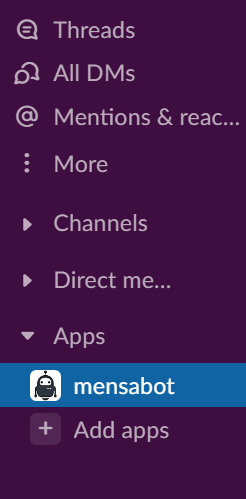
\includegraphics[height=7cm]{bot.png}
% \end{figure}


      
\subsection*{Task 1 - Getting to know the bot}
\subsubsection*{Getting the menu}
\begin{enumerate}
    \item Write a greeting message (e.g. Hello)
    \item You can type \textbf{help} to see a list of the capabilities of the bot
    \item Ask the bot to get the menu for your local mensa (canteen)
    \begin{itemize}
      \item Canteens might be closed
      \item You can also ask the bot about canteens in a particular city (e.g what is the menu for mensas in Aachen?)
      \item Try using Aachen, Mensa Academica or Aachen, Mensa Vita
    \end{itemize}
    \item The bot will look up the menu
    \item The bot might ask you if you want to set a default city. Answer with an appropriate message
\end{enumerate}
\subsubsection*{Make a review}
\begin{enumerate}
    \item Ask the bot to write a review (e.g. I want to add a review)
    \item The review process should now be starting 
    \item The bot will ask you a series of questions
    \item First specify which mensa you went to and which meal you had (e.g. I went to Aachen, Mensa Academica and had the Klassiker) 
    \begin{itemize}
      \item The spelling of the category of the dish must be in the same manner as displayed on the menu (\textbf{Klassiker, Vegetarisch} not classics or vegetarian)
    \end{itemize}
    \item Specify how many stars out of 5 you would give your meal
    \item The bot will ask you to leave a comment
    \begin{itemize}
        \item Leave an appropriate comment
        \item You can also type no if you don't want to leave a comment
      \end{itemize}
\end{enumerate}

\subsection*{Task 2 - Make a visualization}
This task involves getting insights into the success of the community. Certain success measures are predefined, which can be visualized by using the bot. Visualizations can be either a value, a chart, or a ratio.
\begin{enumerate}
    \item Ask the bot to make a visualization (e.g Make a visualization)
    \item The bot will ask for a measure. Ask the bot to list all measures
    \item Choose one of the measures 
    \begin{itemize}
        \item Copy the measure and paste it into the typing field. Then hit ENTER
    \end{itemize}
    \item The bot will respond with the appropriate visualization
    
\end{enumerate}


\subsection*{Task 3 - Update the success model}
This task involves updating the success model of the community. The success model is structured into six success \textbf{dimensions}. Each dimension contains a list of \textbf{factors}. Each factor contains a list of \textbf{measures}, which define the visualizations.
The success model is based on the requirements of the community. Those requirements were collected during the first evaluation.
\begin{enumerate}
    \item Use the bot to get the success model (e.g. Get the success model)
    % \begin{itemize}
    %     \item The bot will now list the different success dimensions
    %     \item Each dimension contains success factors
    %     \item For each factors, different measures can be listed
    % \end{itemize}
    \item Aks the bot to update the success model
    \item The bot will ask you to choose which success dimension you want to edit
    \item Choose a dimension by providing a \texttt{number}
    \item The bot will now ask you which success factor you want to edit
    \item Choose one by providing a \texttt{number} or add one by choosing a name for the factor (e.g. Customer Satisfaction)
    \item Select one of the measures. 
    \item The bot will now add the factor to the model.
    \item You can also visualize your new measure in the same way as described in Task 2
\end{enumerate}

\subsection*{Feedback}
  
\begin{enumerate}
  \item Please fill out the following survey: \url{https://limesurvey.tech4comp.dbis.rwth-aachen.de/index.php/164344?lang=en}
  \item If the link does not work, copy-paste  the one in the footnotes \footnotemark 
  \footnotetext{https://limesurvey.tech4comp.dbis.rwth-aachen.de/index.php/164344?lang=en}
\end{enumerate}


\section{Free text Feedback}

"Buttons would be really nice when choosing which visualization to make. 
When presenting the success model, further text formating would have been nice (e.g. using bold to write the category names).
Maybe more nudging in regards to asking users to use the proposed review, visualize and especially success model extension features. Similarly, maybe add some explanations on the benefits and goals of the success model to the bot. Some users might not immediately get the point of the success models. 
The possibility to change a review or a comment would also be neat. 
Some visualizations which contained the users' email address in the y-axis resulted in a diagram which was not really lined up with the bars.
Overall still a nice and interactive way of asking for the menu and creating communities. Especially when looking at the given use case, one can imagine taking their phone to create such a review or quickly search for the menu before entering the canteen. Especially with the bot being available on one's mobile device and that on a trusted platform. "
\bigbreak
"I like that I can just enter natural language queries to get answers from the bot. It is very good that it always answers quickly. Even if an operation takes longer, it still gives you an initial message to let you know that the bot is still working on providing the answer. I like that the bot has a profile picture. It is very useful to quickly query the menu instead of manually searching it online.
Sometimes, I was not 100\% sure which kind of answer the bot would understand, so whether I could just talk in free text, enter a number of a list or copy a specific list entry. This aspect could be unified a bit more. To visualize a measure, you have to copy its exact name but to update the measure, you can navigate using the numbers. The bot also requires the exact name of the dish category (Klassiker). Here, different alternatives like writing ""classics"" should probably be allowed to increase the user's confidence that the operation is going to succeed.
Adding a review is a bit cumbersome as it requires multiple messages with intermediate waiting periods for the bot's answers. Users would probably prefer if they could enter one message like ""I had the Klassiker and would rate it with 5 stars"" to go through multiple steps at once. After that, the bot could just ask for confirmation of all information at once."
\bigbreak
"Once, I started with one request, the bot did not find another request, when I wanted to quit the first request and to start a new one. I would have been nice, if the bot immediately change to the new request instead of giving out a error message."
\bigbreak
"Sometimes the bot gave an answer right away, even if it just was telling you to wait a second. I liked this very much, as it gave me a very responsive experience. I would wish for the bot to always give such an answer, when having to compute visualizations or the success model, just so I know it heard me and will eventually response."
\bigbreak
"Bots are hard to use, in comparison to normal interface, and not fun at all"
\bigbreak
"The presentation was well done and was understandable."
\bigbreak
"When the bot gave a numbered list of mensas, I entered a number  (5), but the bot gave information for another number (2).
A lot of listed mensas didn't work, or were not recognised.
I had to pay attention how to write commands, e.g. city before mensa, not the other way around. The commands could be more universal.
On the plus side, the visualisation was good."
\bigbreak
"the functionalities seem to be all around well integrated with the chatbot and the intent recognition seems to be very good"
\bigbreak
"-clickable list for different tasks.\newline
-favorise ones Mensa, not only cities."
\bigbreak
"It's pretty self explainatory, except the success model part."
\bigbreak
"There's a general lack of feedback after commands."

\section{System Usability Scale}
\begin{figure}[H] 
    \begin{center}
    \begin{tikzpicture}
      \begin{axis}
        [xmin=0.9,xmax=5.1,
        height=20cm,width=9cm,ytick={1,2,3,4,5,6,7,8,9,10},
                        label style={font=\footnotesize},
                        tick label style={font=\footnotesize}, yticklabel style={align=right},ylabel={Average User Rating (N=20)},
        yticklabels={I needed to learn a lot of things\\ before I could get going with\\ the system.,I felt very confident using \\the system. , I found the system very cumbersome to use. ,I would imagine that most people\\ would learn to use the system very quickly. ,I thought there was too\\ much inconsistency in the \\system. ,I found the various functions\\ in the system\\ were well integrated. ,I think that I would need the\\ support of a technical person to \\be able to use the system. ,I thought the system\\ was easy to use. ,I found the system\\ unnecessarily complex. ,I think that I would like to \\ use this system frequently.},scatter/classes={
      a={mark=*,red!50!black},
      b={mark=*,blue!50!black},
      c={mark=*,green!50!black},
      d={mark=*,white!50!black}
     }]
        \addplot[color=blue,
        boxplot prepared={
            median= 2,
          upper quartile=3,
          lower quartile=1,
          upper whisker=5,
          lower whisker=1
        },
         ] coordinates {}; 
        \addplot[color=blue,
        boxplot prepared={
            median= 4,
          upper quartile=5,
          lower quartile=3,
          upper whisker=5,
          lower whisker=2
        },
         ] coordinates {}; 
        \addplot[color=blue,
        boxplot prepared={
            median= 2,
          upper quartile=3,
          lower quartile=1,
          upper whisker=5,
          lower whisker=1
        },
         ] coordinates {}; 
        \addplot[color=blue,
        boxplot prepared={
            median= 4,
          upper quartile=5,
          lower quartile=3,
          upper whisker=5,
          lower whisker=2
        },
         ] coordinates {}; 
        \addplot[color=blue,
        boxplot prepared={
            median= 2,
          upper quartile=3,
          lower quartile=1,
          upper whisker=5,
          lower whisker=1
        },
         ] coordinates {}; 
        
     \addplot[color=blue,
        boxplot prepared={
            median= 4,
          upper quartile=5,
          lower quartile=4,
          upper whisker=5,
          lower whisker=3
        },
         ] coordinates {}; 
        \addplot[color=blue,
        boxplot prepared={
            median= 1,
          upper quartile=2,
          lower quartile=1,
          upper whisker=5,
          lower whisker=1
        },
         ] coordinates {}; 
         \addplot[color=blue,
        boxplot prepared={
            median= 4,
          upper quartile=5,
          lower quartile=3,
          upper whisker=5,
          lower whisker=1
        },
         ] coordinates {}; 
         \addplot[color=blue,
        boxplot prepared={
            median= 2,
          upper quartile=2,
          lower quartile=1,
          upper whisker=5,
          lower whisker=1
        },
         ] coordinates {}; 
         \addplot[color=blue,
        boxplot prepared={
            median= 4,
          upper quartile=5,
          lower quartile=3,
          upper whisker=5,
          lower whisker=1
        },
         ] coordinates {}; 
         \addplot[scatter,only marks,scatter src=explicit symbolic] 
            table [
                y=y,
                x=x
                ]
            {
            x y 
            2 1 
            4 2 
            2 3 
            4 4
            2 5
            4.5 6
            1.5 7
            4 8
            1.5 9
            4 10
            };
    \node[align=center, text=black]
    at (axis cs:4 ,10.2) {\scalebox{0.8}{SD=1.25}};
    \node[align=center, text=black]
    at (axis cs:1.5,9.2) {\scalebox{0.8}{SD=1.23}};
    \node[align=center, text=black]
    at (axis cs:4 ,8.2) {\scalebox{0.8}{SD=1.3}};
    \node[align=center, text=black]
    at (axis cs:1.5 ,7.2) {\scalebox{0.8}{SD=1.08}};
    \node[align=center, text=black]
    at (axis cs:4.5 ,6.2) {\scalebox{0.8}{SD=0.69}};
    \node[align=center, text=black]
    at (axis cs:2 ,5.2) {\scalebox{0.8}{SD=1.28}};
    \node[align=center, text=black]
    at (axis cs:4 ,4.2) {\scalebox{0.8}{SD=0.91}};
    \node[align=center, text=black]
    at (axis cs:2 ,3.2) {\scalebox{0.8}{SD=1.3}};
    \node[align=center, text=black]
    at (axis cs:4 ,2.2) {\scalebox{0.8}{SD=1.01}};
    \node[align=center, text=black]
    at (axis cs:2 ,1.2) {\scalebox{0.8}{SD=1.22}};
      \end{axis}
    \end{tikzpicture}
    \end{center}\caption{Results of SUS Statements}
        \label{fig:SusPlot}
\end{figure}
\end{appendices}
